\documentclass{standalone}

%----------------------------------------------------------------------------------------------%
%                                 Packages and basic declarations
%----------------------------------------------------------------------------------------------%

\usepackage[utf8]{inputenc}
\usepackage{pgfplots}
\usepackage{tikz}


%----------------------------------------------------------------------------------------------%
%----------------------------------------------------------------------------------------------%
%                                            DOCUMENT STARTS
%----------------------------------------------------------------------------------------------%
%----------------------------------------------------------------------------------------------%

\begin{document}


%Tikz picture starts%

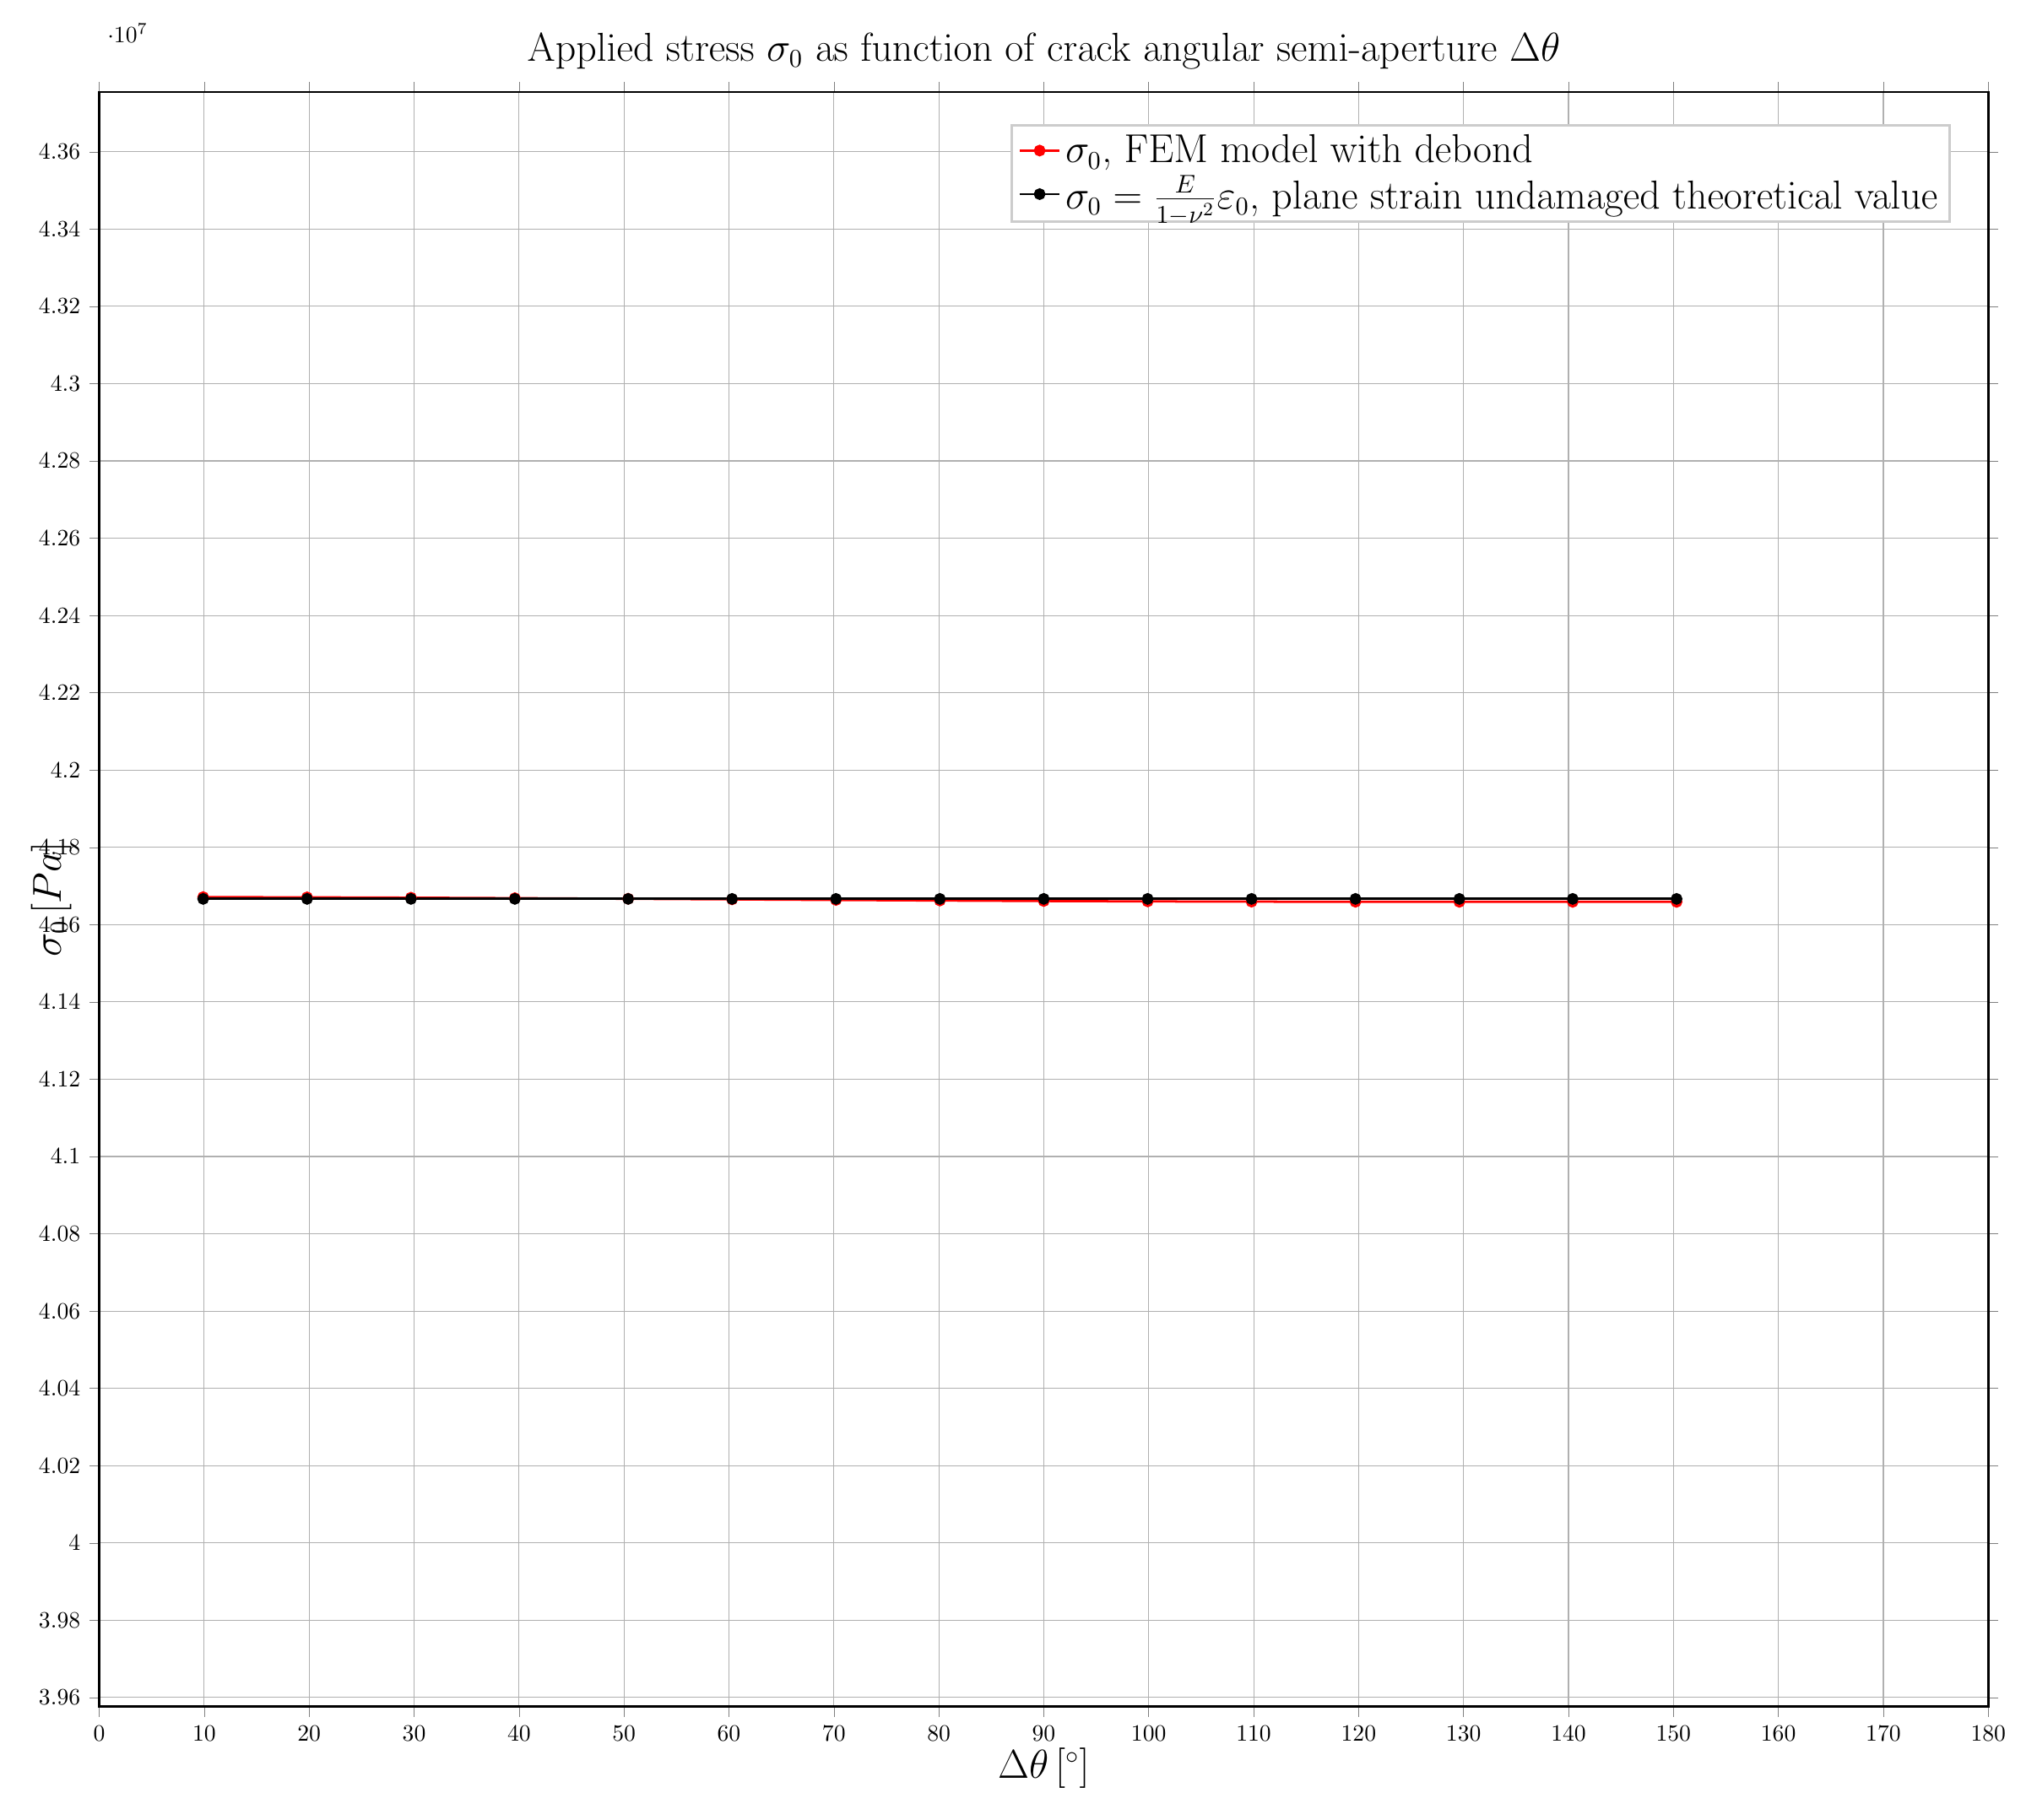
\begin{tikzpicture}

%Tikz axis starts%

\begin{axis}[width=30cm,
title={Applied stress $\sigma_{0}$ as function of crack angular semi-aperture  $\Delta\theta$},
title style={font=\fontsize{16}{8}\selectfont},
xlabel style={at={(axis description cs:0.5,-0.02)},anchor=north,font=\fontsize{16}{8}\selectfont},
ylabel style={at={(axis description cs:-0.01,.5)},anchor=south,font=\fontsize{16}{8}\selectfont},
xlabel={$\Delta\theta\left[^{\circ}\right]$},ylabel={$\sigma_{0}\left[Pa\right]$},
xmin=0.0,
xmax=180.0,
ymin=39576059.957,
ymax=43754835.3167,
tick align=outside,
tick label style={font=\normalsize},
xtick={0.0,10.0,20.0,30.0,40.0,50.0,60.0,70.0,80.0,90.0,100.0,110.0,120.0,130.0,140.0,150.0,160.0,170.0,180.0},
xmajorgrids,
x grid style={lightgray!92.026143790849673!black},
ymajorgrids,
y grid style={lightgray!92.026143790849673!black},
line width=0.35mm,
legend style={draw=white!80.0!black,font=\fontsize{16}{12}\selectfont},
legend entries={{$\sigma_{0}$, FEM model with debond},{$\sigma_{0}=\frac{E}{1-\nu^{2}}\varepsilon_{0}$, plane strain undamaged theoretical value}},
legend cell align={left}
]

\addplot[red,smooth,mark=*]
table{
9.90004415946 41671271.7302
19.800125885 41670679.3568
29.700111134 41669739.5249
39.5999409963 41668519.5583
50.4000580931 41666965.1447
60.2998879554 41665435.3567
70.1998714969 41663898.7513
80.0999574912 41662451.3758
90.0000025045 41661202.2513
99.9000475177 41660239.3424
109.800126682 41659593.2045
119.700103393 41659229.1086
129.599943501 41659071.2897
140.400057182 41659026.703
150.29988363 41659023.7948
};

\addplot[black,smooth,mark=*]
table{
9.90004415946 41666666.6667
19.800125885 41666666.6667
29.700111134 41666666.6667
39.5999409963 41666666.6667
50.4000580931 41666666.6667
60.2998879554 41666666.6667
70.1998714969 41666666.6667
80.0999574912 41666666.6667
90.0000025045 41666666.6667
99.9000475177 41666666.6667
109.800126682 41666666.6667
119.700103393 41666666.6667
129.599943501 41666666.6667
140.400057182 41666666.6667
150.29988363 41666666.6667
};

\end{axis}
%Tikz axis ends%


\end{tikzpicture}
%Tikz picture ends%


\end{document}

%----------------------------------------------------------------------------------------------%
%----------------------------------------------------------------------------------------------%
%                                            DOCUMENT ENDS
%----------------------------------------------------------------------------------------------%
%----------------------------------------------------------------------------------------------%

